\chapter{Methods} \label{chapter:methods}
% This chapter introduces the methods we developed.
% We start with the \ac{GLD} algorithm and through constant 
% empirical testing propose modifications to overcome its
% limitations on problem size. 
% Our final goal is to fine-tune \iac{LLM} using 
% the modified algorithm such that we can study 
% the effectiveness of direct search methods in 
% optimizing large neural networks and the possibility 
% to use a direct search method as a memory-efficient 
% alternative to first-order gradient-based optimization
% techniques.

We start with the \ac{GLD} algorithm \parencite{gld} 
and through constant 
empirical testing propose modifications to overcome its
limitations. Our goal is to 
develop a memory-efficient method
that can perform comparably to 
state-of-the-art first-order gradient-based optimization
techniques when fine-tuning \iac{LLM}.
We understand that such a method might come at the 
cost of increased
time complexity, particularly considering the 
already established slow convergence rates of direct 
search methods \parencite{directsearch}. 
Nevertheless, we try to find a balance
such that convergence rates remain reasonable.  
This chapter introduces the modifications we developed.

\section{Parameter Partitioning}\label{section:partitioning}
The biggest hurdle to fine-tuning \iac{LLM} using 
direct search methods is the problem size. \acp{LLM}
have a large number of parameters, 
% which means training
% them all at the same time goes beyond the capabilities of 
% our base algorithm. 
which means training them all at the same time 
is impractical with our base algorithm as it would 
have to use very small radii. 
Instead, we divide the parameters into
subsets and we let 
the \ac{GLD} algorithm optimize one subset at a time. 

Initially, we experimented with considering each individual weight matrix and
bias vector of the network as one subset. 
% We quickly realize that some weight matrices are still too 
% large on their own even after the partitioning. 
However, this partitioning scheme proved to be too 
coarse since some weight matrices were still too large 
on their own even after the partitioning.
For those
weight matrices we develop different methods to 
select $s$ individual weights
to train at each iteration, where $s$ is a number of variables
optimizable by \ac{GLD}. The simplest method
is to select $s$ weights at random. We mainly use this 
method for our experiments. We also experiment with 
picking weights based on importance where we 
rank the weights based on some importance
metric and select the $s$ elements with the highest ranking. 
We consider two different importance metrics: the absolute
value and the Fisher importance. 

The absolute value 
method comes from the intuition that higher absolute 
weight values have a more noticeable effect on the output of a layer
(Conversely, weights close to 0 
have little effect). 

The Fisher method requires
estimating the  as described \ac{FIM}
in \autoref{section:fisher}. This is a costly process,
making it infeasible to run in each iteration. Instead,
we run it only a few times 
throughout the entire training. See 
\autoref{section:partition} for the details 
of our experiments. 

% We also allow 
% a custom function to select different intervals of size $s$ 
% from the 
% list of weights sorted on importance instead of constantly
% picking the first $s$ weights. 
% We take this approach to be crucial for the potential success
% of the Fisher method 
% because even if the Fisher information estimate accurately
% determines the importance of weights,  
% training only the same $s$ 
% weights at all times when $s$ is significantly smaller
% than the size of the matrix 
% means a big part of the weight matrix
% remains untouched, which assumably would have
% a negative impact on performance.

As an initialization step, we assign each tensor 
that needs further reduction in size one of the defined 
methods (random, absolute value or Fisher) 
to select the parameters 
that are to be trained in an iteration.
Each iteration $t$ selects a list of perturbation indices $\mathbf{i}$
for each tensor $\bm{\theta}$.
The tensor is then perturbed by vector $\mathbf{v}$ with
$\bm{\theta}_t(\mathbf{i}) = \bm{\theta}_t(\mathbf{i}) + \mathbf{v}$
where $\bm{\theta}_t(\mathbf{i})$ refers to parameters 
of the tensor at indices $\mathbf{i}$. 
Matrices, which comprise 
$\leq s$ parameters receive updates for all their 
parameters. Similarly, 
we can assign each tensor a maximal radius 
$R$ for the binary search of \ac{GLD}, allowing 
the flexibility to search
in different intervals for different parameters. 
In the following,  
$R(\bm{\theta})$ denotes the maximal radius assigned to 
a tensor $\bm{\theta}$.
In this case, we consider the number of used radii $K$ 
as a tunable hyperparameter of 
the algorithm instead of providing the minimal radius $r$.
The search interval can then be described as 
$[2^{1-K}R, R]$.

\begin{algorithm} 
    \caption{\acl{GLD} Training}
    \label{algorithm:main}
    \begin{algorithmic}[1]
        \For{$t=1, \dots, T$}
        % \State $x, y \gets$ \Call{GetMinibatch}{}
        \ForAll{tensor $\bm{\theta}_t$}
        \State $\mathbf{i} \gets $ \Call{SelectPerturbationIndices}{$\bm{\theta}_t$, $s$}
        \Comment{Either selects all indices, or selects $s < \textrm{size}(\theta_t)$
        indices using one of our random, absolute value or Fisher methods}
        % \State $\theta_{t, \textrm{train}} \gets$ \Call{PickParametersToTrain}{$\theta_t$}
        \For{$k = 1, \dots, K$}
        \State $r_k \gets 2^{-k}R(\bm{\theta}_t)$
        \State $\mathbf{v}_k \sim r_k \mathcal{D}$
        % \State $\bm{\theta}_{t, k} \gets$ \Call{Perturb}{$\bm{\theta}_t$, $v_k$}
        \State $\bm{\theta}_{t, k} \gets \bm{\theta}_t$
        \State $\bm{\theta}_{t,k}(\mathbf{i}) \gets \bm{\theta}_{t,k}(\mathbf{i}) + \mathbf{v}_k$
        \EndFor
        % \State $\bm{\theta}_{t+1} \gets \arg \min_k \{\mathcal{J}(\bm{\theta}; x, y)|\bm{\theta} = \bm{\theta}_t, \bm{\theta}=\bm{\theta}_{t,k}\}$ 
        \State $\bm{\theta}_{t+1} \gets \arg \min_{\bm{\theta}} \{\mathcal{J}(\bm{\theta}_t), \mathcal{J}(\bm{\theta}_{t,k})\}$ 
        \EndFor
        \EndFor
    \end{algorithmic}
\end{algorithm}

\autoref{algorithm:main} defines our main method for
training neural networks using \ac{GLD}. Since it is 
crucial to reduce the size of the problem to
successfully apply \ac{GLD}, all
further methods we define also partition parameters as 
in \autoref{algorithm:main}. 

\section{Radius scheduling}
% The radius $r_k$ in \autoref{algorithm:main} 
% determines how big the values 
% are in the perturbation vector $\mathbf{v}_k$. 
% Thus, it determines
% the step size when $\mathbf{v}_k$ is the perturbation 
% that gives 
% the best loss. 
The radius $r_k$ in \autoref{algorithm:main} 
serves a similar purpose as the step size 
when the perturbation vector
$\mathbf{v}_k$ gives the best loss, as 
together with the distribution $\mathcal{D}$, 
it determines how big the values are in $\mathbf{v}_k$. 
It is therefore comparable to the learning
rate of first-order optimizers. 

As discussed in \autoref{section:directsearch}, the 
binary search performed by \ac{GLD} 
across the interval $[r, R]$
makes it possible to give
convergence guarantees depending
on the values of $r$ and $R$. Better guarantees
can be given for bigger search intervals as the algorithm
considers both large radii to escape saddle points
and small radii to converge when in a close neighborhood
of the minimum. However, having a large search interval 
also increases the number of forward passes required
in each iteration, increasing the time complexity 
of the algorithm. Ideally, we want to keep $K$ small 
without sacrificing the ability to converge. 

The resemblance between search radius and learning rate 
brings about the idea to implement a radius 
scheduler similar to a learning rate scheduler for 
first-order optimizers. We already assigned each parameter
matrix a maximal radius $R$. We extend our implementation 
to assign each tensor a radius scheduler as well.
A scheduler is hereby a function 
$\mathbb{R} \rightarrow \mathbb{R}$ taking 
the current step count and returning a multiplier 
for $R$. With constant $K$, this is 
equivalent to shifting the interval $[r, R]$ 
during training. Starting with larger radii and 
gradually shifting the interval towards smaller radii,
we expect to keep the base algorithm's convergence
with a fewer number of forward passes each iteration. 

\section{Options}
A key weakness of \autoref{algorithm:main} is that 
updates through random perturbation of parameters end up
being noisy. Often, a perturbation that improves 
the objective for one mini-batch makes it worse 
for others. A stabler update policy is desired as it could
allow faster progress and better convergence. The simplest
way to solve this issue is to increase the batch size, 
making it more likely for perturbations picked by the 
algorithm to be good in the long run. In this section
we introduce a different approach. We store so-called
\textit{options}, potential updates 
that the algorithm has considered for each tensor,
and update to an option only after exploring a lookahead
of future updates it can lead to. 

We define an option $p$ as a tuple $(\mathbf{i}, \mathbf{v})$ of indices 
and perturbation vector that stores a perturbation 
applied by the algorithm. With $\bm{\theta}_p$, we denote a 
tensor resulting from perturbing according to $p$.
Similarly $\bm{\theta}_{t,p}$ denotes the tensor at time
step $t$ being perturbed according to $p$. 
For each tensor $\bm{\theta}$ 
we define a set of options $\psi(\bm{\theta})$. 
After the binary search, the algorithm does not update 
the parameter with the best perturbation. Instead the 
top $m$ candidates are stored in $\psi(\bm{\theta})$. 
In each iteration $t$, the algorithm then applies each 
option $p \in \psi(\bm{\theta}_t)$ and does a binary search for 
perturbations on each $\bm{\theta}_{t, p}$. We say
$p^* \in \psi(\bm{\theta}_t)$ is the best option if one of the 
perturbations on $\bm{\theta}_{t,p^*}$ gives the 
minimum objective of that step. The parameter is updated
to $\bm{\theta}_{t,p^*}$ and $\psi(\bm{\theta}_{t+1})$ is produced 
from the top $m$ perturbations on $\bm{\theta}_{t,p^*}$.
We note that for $m=1$ the method is equivalent to 
\autoref{algorithm:main}: Since there is only one option,
$p^*$ is always the best perturbation found in an iteration 
and the next iteration will update the parameter with $p^*$.

The method can be extended to include multiple 
layers of options. In that case, each option $p$ also 
stores a set of options $\psi(p)$. We refer to the number of 
option levels as $\ell$. 
\autoref{figure:optionstree} visualizes two levels of 
options on a tensor. 
This setup can be 
understood as a tree structure with a height of $\ell$ where 
each level has a width of $m$ and each node holds an 
option. At the root of the tree is 
the parameter $\bm{\theta}$, which can be described as an 
"empty" option where the perturbation vector is 0.
$\psi(p)$ describes the children of each node and
we have $\psi(p) = \emptyset$ for leaf nodes, which are 
options at the $\ell$-th level.

\begin{figure}
    \centering
    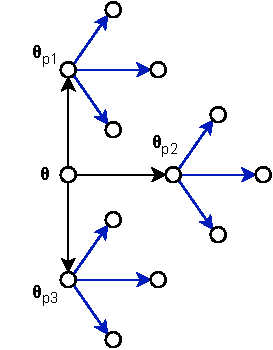
\includegraphics{figures/options.pdf}
    \caption[Visualization of two levels of options]
    {Visualization of a potential setup of 
    two levels of options.
    Black and blue arrows show 
    first-level and second-level options respectively. 
    $K$ perturbations are applied on each option on the 
    second level and $\bm{\theta}$ is updated to 
    either $\bm{\theta}_{p1}$,
    $\bm{\theta}_{p2}$ or $\bm{\theta}_{p3}$
    depending on which
    first-level option is the parent of the 
    best perturbation.
    }
    \label{figure:optionstree}
\end{figure}

\autoref{algorithm:options} gives the formal definition
of the method. 
Intuitively, the proposed method describes 
a lookahead into 
potential future updates from each point to select 
parameter updates 
which provide a continuous loss decrease 
over multiple steps.
An update is selected if one of its updates 
at the $\ell$-th level
gives the best objective. 
We hypothesize this will reduce the noise of
updates.

We remark that the type of lookahead we develop is in 
essence only slightly different to applying 
\autoref{algorithm:main} with larger batch sizes: When 
performing a single parameter update,
\autoref{algorithm:options} considers 
not only multiple mini-batches but also multiple
perturbations on the original parameter. We can say 
with batch size $b$, 
$(\ell+1) \cdot b$
samples and $\sum_{i=0}^\ell m^i \cdot K$ perturbations 
influence a parameter update, while each 
perturbation considers $b$ samples and from each point we 
have $K$ perturbations. We can look ahead to points up to 
$(\ell+1) \cdot R$ optimization steps away from the original parameter 
but each perturbation is still in the interval $[r, R]$.
Using options significantly increases the number 
of forward passes performed in each iteration with
$m^\ell \cdot K$ forward passes per tensor 
instead of only $K$. However, unlike using a larger 
batch size, any improvement in 
performance comes at no additional memory cost.  

\begin{algorithm} 
    \caption{\acl{GLD} Training with Options}
    \label{algorithm:options}
    \begin{algorithmic}[1]
        \For{$t=1, \dots, T$}
        % \State $x, y \gets$ \Call{GetMinibatch}{}
        \ForAll{tensor $\bm{\theta}_t$}
        % \State $\bm{\theta}_{t, \textrm{train}} \gets$ \Call{PickParametersToPerturb}{$\bm{\theta}_t$}
        % \ForAll{$p \in \psi(\bm{\theta}_t)$}
        % \State $\mathcal{J}(\bm{\theta}_{t, p}) \gets $ \Call{ComputeOptionLoss}{$\bm{\theta}_t$, $p$}
        % \EndFor
        \State $\mathbf{i} \gets $ \Call{SelectPerturbationIndices}{$\bm{\theta}_t$, $s$}
        \State $p^* \gets \arg \min_{p \in \psi(\bm{\theta}_t)} \{$\Call{ComputeOptionLoss}{$\bm{\theta}_t$, $p$, $\mathbf{i}$}$\}$ 
        \Comment{Best first-level option}
        \State $\bm{\theta}_{t+1} \gets \bm{\theta}_{t,p^*}$ 
        \State $\psi(\bm{\theta}_{t+1}) \gets \psi(p^*)$
        \EndFor
        \EndFor
        \Procedure{ComputeOptionLoss}{$\bm{\theta}_t$, $p$, $\mathbf{i}$}
        % \State $\bm{\theta}_{t,p} \gets$\Call{ApplyOption}{$\bm{\theta}_t$, $p$}
        \If{$\psi(p) = \emptyset$}
        \LComment{If this is the last level of options, apply perturbations to set the next level and return the minimum loss}
        \For {$k=1, \dots, K$}
        \State $r_k \gets 2^{-k}R(\bm{\theta}_t)$
        \State $\mathbf{v}_k \sim r_k \mathcal{D}$
        \State $\bm{\theta}_{t,p,k} \gets \bm{\theta}_{t,p}$
        \State $\bm{\theta}_{t,p,k}(\mathbf{i}) \gets \bm{\theta}_{t,p,k}(\mathbf{i}) + \mathbf{v}_k$ 
        \EndFor
        % \State $\mathcal{J} \gets \min_k\{\mathcal{J}(\bm{\theta}; x, y) | \bm{\theta} = \bm{\theta}_{t, \textrm{perturb}} , \bm{\theta} = \bm{\theta}_{t, \textrm{perturb}} + v_k\}$
        \State $\psi(p) \gets \arg\min_{p'}^{(m)}\{\mathcal{J}(\bm{\theta}_{t,p,p'}) \mid p' \in \{(\mathbf{i}, \mathbf{0}), (\mathbf{i}, \mathbf{v}_k) \mid k = 1, \dots K\}\}$
        \Comment{The top $m$ candidates}
        \State \Return $\min_k\{\mathcal{J}(\bm{\theta}_{t,p}), \mathcal{J}(\bm{\theta}_{t,p,k})\}$
        \Else
        \LComment{If this is not the last level of options, recursively return the minimum loss across all children}
        \State \Return $\min_{p' \in \psi(p)}\{$\Call{ComputeOptionLoss}{$\bm{\theta}_{t,p}$, $p'$, $\mathbf{i}$}$\}$
        % \State $\mathcal{J} \gets \infty$
        % \ForAll{child $p'$}
        % \State $\mathcal{J} \gets \min_{p' \in \textrm{children}(p)}\{\mathcal{J},$ \Call{ComputeOptionLoss}{$
        % _{t,p}$, $p'$}$\}$
        % \EndFor
        \EndIf
        % \State \Return $\mathcal{J}$
        \EndProcedure
    \end{algorithmic}
\end{algorithm}

% \section{Accelerated Forward Passes}
% Unlike first-order methods, our algorithm requires 
% multiple forward passes per iteration to update 
% parameters. To speed up the process,  
% \section{Weight Decay}

% \section{Implementation Details}
% % fast forward
% % give k instead of r, constant k 